\documentclass{beamer}
\usetheme{Boadilla}
\usecolortheme{seahorse}
\usefonttheme{serif}

\usepackage{lipsum}
\usepackage{graphicx,xcolor}
\usepackage{amsmath,amssymb,amsfonts}

\AtBeginSection[]{ 
    \begin{frame}{Outline} 
        \tableofcontents[currentsection] 
    \end{frame} }

\title[Waterfall Method]{Software project management methods:}
\subtitle{The waterfall method}
\author[]{ Sacha Alidadi Heran \\ Diana Fonseca \\ Nick Ecker \\ Iman Barkan}
\institute[Projet, Master 1 CSMI]{}
\titlegraphic{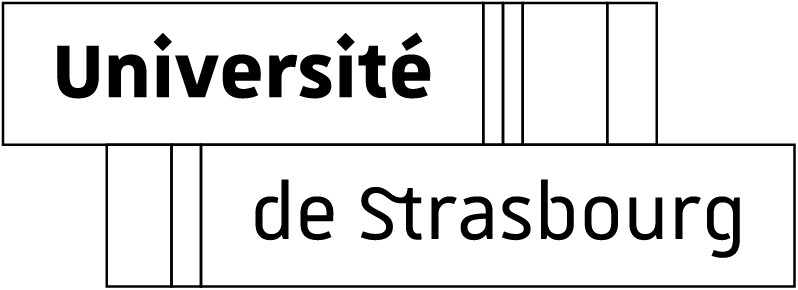
\includegraphics[width=0.3\textwidth]{images/logo/unistra.jpg}}
\date{31/01/2023}


\begin{document}

\begin{frame}
\titlepage
\end{frame}


\section{Introduction}
\subsection{Overview of the method}
\begin{frame}{Introduction}

   \begin{block}{Overview of the method}

   \item Waterfall methodology, also known as Waterfall model is a linear process model used in project management

   \item Sequential process divided into phases
   
   \item Each phase must be completed before the next one can begin

   \item Outputs of each phase are used as inputs for the next phase

   \item After their completion, a phase can't be revisited

   \item Best adapted to projects with well-defined requirements

   \end{block}

\end{frame}

\begin{frame}{Introduction}

   \begin{block}{Histoire}

   \item First description of a Waterfall model was in 1956 for the development of the software SAGE

   \item First detailed diagram of this process was introduced by Winston Walker Royce in 1970

   \item First use of the term "Waterfall" was around 1976

   \item Initially the model comes from the construction industry

   \end{block}

\end{frame}



\section{Stages of the Waterfall method}
\subsection{Requirements gathering and analysis}
\subsection{Design}
\subsection{Implementation}
\subsection{Testing}
\subsection{Deployment and maintenance}
\begin{frame}{Stages of the Waterfall method}

    \begin{block}{Methodology}
        - A sequential approach to software development (Linear SDLC) 
        
        - Proceeds in distinct phases, with each phase needing to be completed before moving on to the next one.
    \end{block}   

    \begin{figure}
    \centering
    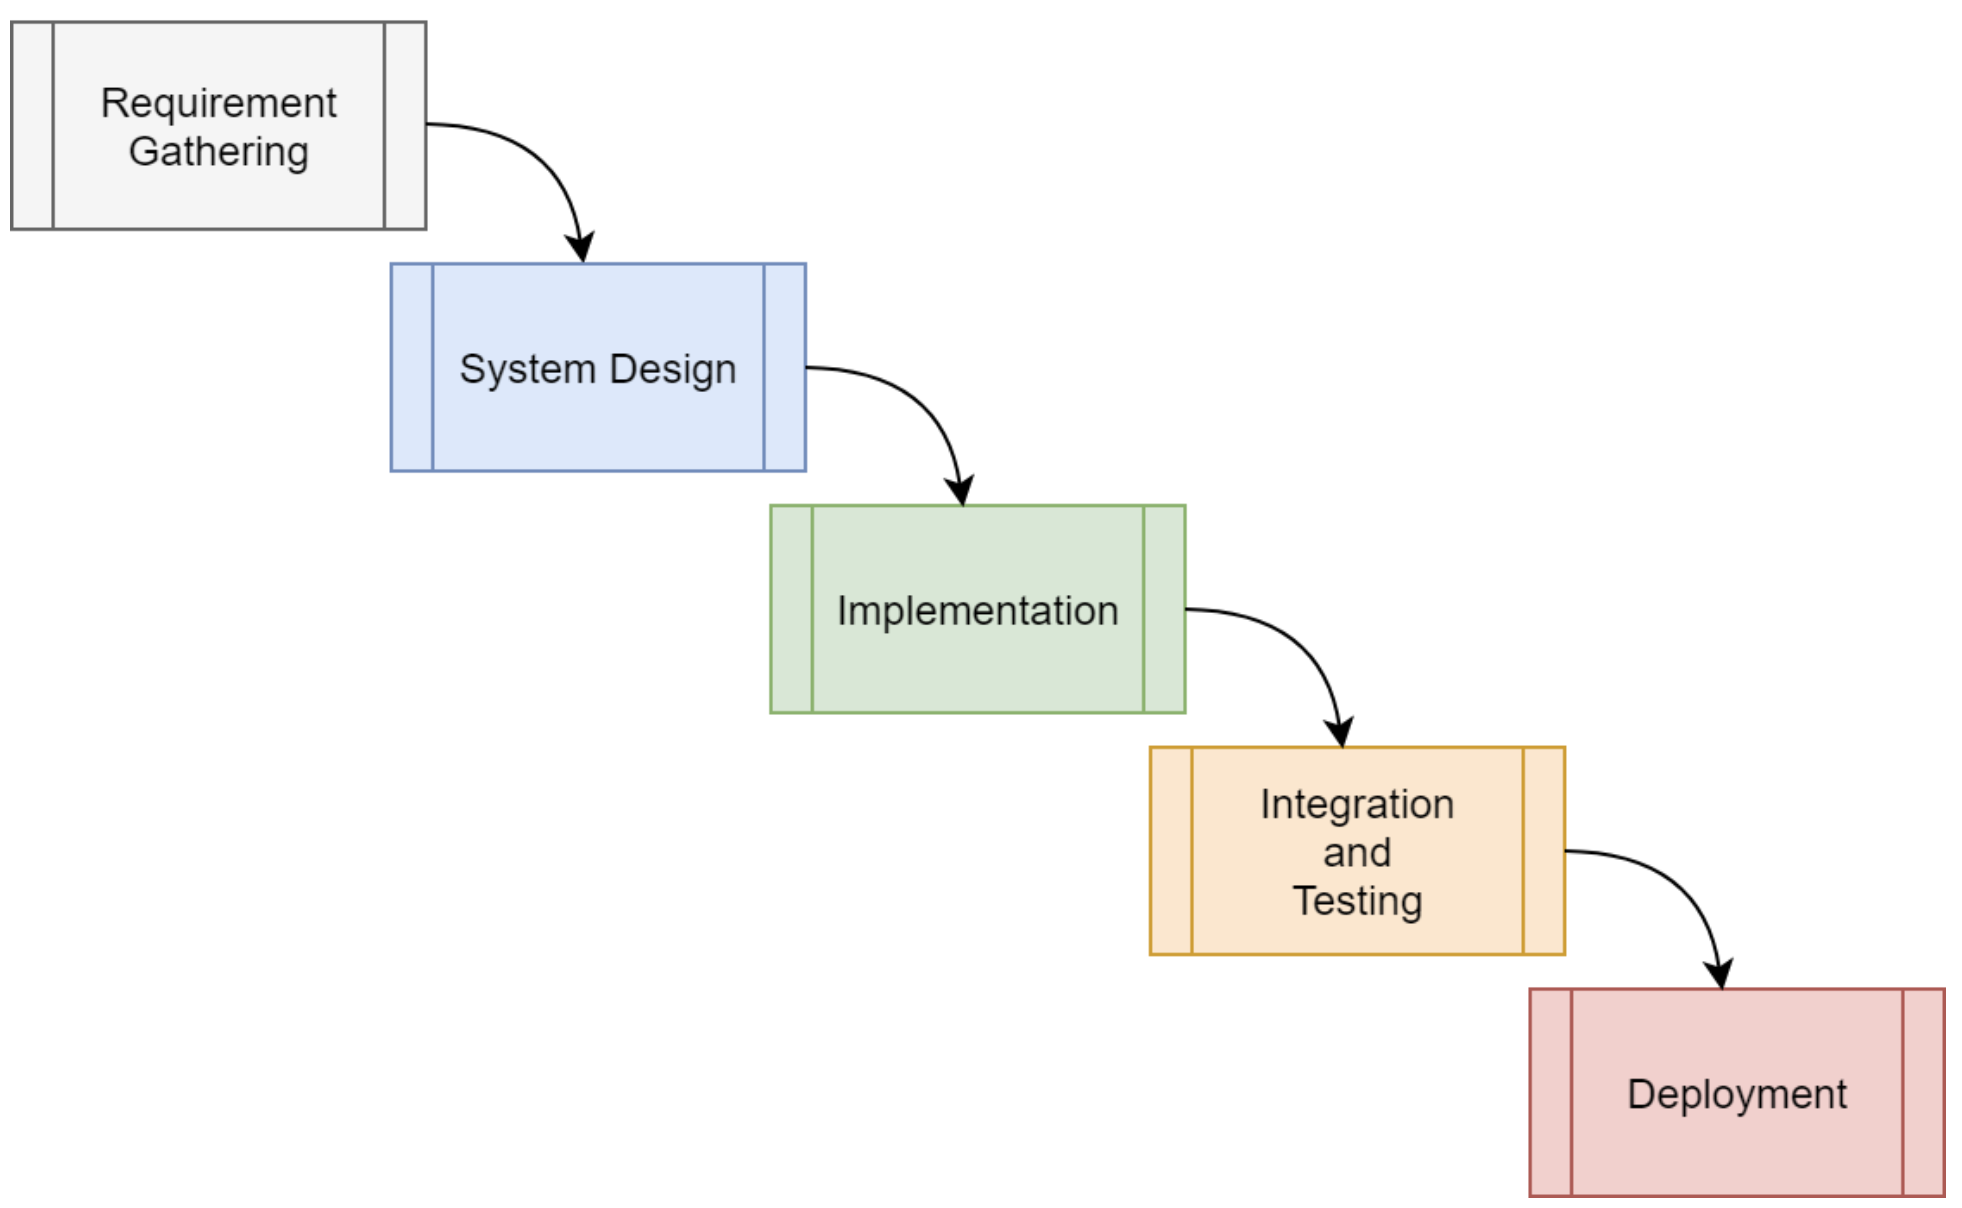
\includegraphics[scale=0.2]{images/illustrate/model.png}
    \caption{Waterfall Model}
    \end{figure}
    
\end{frame}
\begin{frame}{Stages of the Waterfall method}
requirement gathering analysis
    \begin{block}{This is a block}
        \lipsum[1][1-3]
    \end{block}   
    \begin{alertblock}{This is an alert block}
        \lipsum[2][2-5]
    \end{alertblock}  
\end{frame}
\begin{frame}{Stages of the Waterfall method}
design
    \begin{block}{This is a block}
        \lipsum[1][1-3]
    \end{block}   
    \begin{alertblock}{This is an alert block}
        \lipsum[2][2-5]
    \end{alertblock}  
\end{frame}
\begin{frame}{Stages of the Waterfall method}

    \begin{block}{Implementation}
        - Involves actual coding and building of the software
        
        - Close collaboration between development team and stakeholders
        
        - Regular testing and debugging performed to identify and fix issues
        
        - Marks the transition from planning and design to actual software creation
        
    \end{block}   

\end{frame}
\begin{frame}{Stages of the Waterfall method}
testing
    \begin{block}{This is a block}
        \lipsum[1][1-3]
    \end{block}   
    \begin{alertblock}{This is an alert block}
        \lipsum[2][2-5]
    \end{alertblock}  
\end{frame}
\begin{frame}{Stages of the Waterfall method}
    \begin{block}{Deployment and Maintenance}
        - Involves making the software available to end-users 
        
        - Software deployed to the production environment
        
        - Deployment process carefully managed to minimize disruptions and ensure a smooth transition
        
        - Development team provides ongoing maintenance and support
        
        - Fixes bugs, updates software to address changing requirements,
        
        - Ongoing process that continues even after initial release
        
        - Critical to the success of the software and helps ensure it remains useful and relevant over time.
    \end{block}   

\end{frame}

\section{Advantages and limitations}
\subsection{Examination of the benefits and drawbacks of the Waterfall method}
\begin{frame}{Stages of the Waterfall method}    
    \begin{exampleblock}{Advantages}
        \item It provides a clear set of processes that must be followed.
        
        \item There has to be a planning and documentation step.
        
        \item It emphasizes on quality and completeness.
        
        \item Is the ideal for projects that have a clear scope, well-defined requirements.
        
        \item Predictability is key.
     
    \end{exampleblock}

    \end{frame}

\begin{frame}{Stages of the Waterfall method}
    \begin{alertblock}{Limitations}
        \item It relies heavily on detailed upfront planning.
               
        \item The sequential order of the stages makes it difficult to identify and fix problems early on.
        
        \item It is inflexible, which can be a disadvantage in dynamic environments.
        \
        \item It can result in missed requirements if the planning is not thorough enough from the beginning.
        
        \item Testing and debugging are not integrated into the process.
        
    \end{alertblock}
    \end{frame}

\section{Use of Waterfall in Real World}
\subsection{Discussion of a project that used the Waterfall method}
\subsection{Outcome and Lessons Learned}
\begin{frame}{Use of Waterfall in Real World}
Discussion of a project that used the Waterfall method
    \begin{exampleblock}{This is an example block}
        \lipsum[5][1-3]
    \end{exampleblock}
\end{frame}
\begin{frame}{Use of Waterfall in Real World}
Outcome and Lessons Learned
    \begin{exampleblock}{This is an example block}
        \lipsum[5][1-3]
    \end{exampleblock}
\end{frame}

\section{Waterfall vs Agile}
\subsection{Comparison of the Waterfall method to Agile}
\begin{section}{Waterfall vs Agile}

\end{section}



\section{Conclusion}
\subsection{Recap of the Waterfall method}
\subsection{Final thoughts and recommendations}
\begin{frame}{Conclusion}
Recap of the Waterfall method
    \begin{exampleblock}{This is an example block}
        \lipsum[5][1-3]
    \end{exampleblock}
\end{frame}
\begin{frame}{Conclusion}
    Final thoughts and recommendations
        \begin{block}{Process recap}
            5 steps of the Waterfall method:
            
            \begin{itemize}
                \item Requirements
                \item Design
                \item Implementation
                \item Testing
                \item Maintenance
            \end{itemize}
        \end{block}
    \end{frame}


\section*{References}
\begin{frame}
    \frametitle{References}
    \bibliographystyle{amsalpha}
    \bibliography{ref.bib}
\end{frame}

\end{document}
